\documentclass[a4paper, 10pt, ]{article}

\usepackage[slovak]{babel}

% ------------------------------

\usepackage[utf8]{inputenc}
\usepackage[T1]{fontenc}

\usepackage[left=4cm,
            right=4cm,
            top=2.1cm,
            bottom=2.6cm,
            footskip=7.5mm,
            twoside,
            marginparwidth=3.0cm,
            %showframe,
            ]{geometry}

\usepackage{graphicx}
\usepackage[dvipsnames]{xcolor}
% https://en.wikibooks.org/wiki/LaTeX/Colors

% ------------------------------

\usepackage{lmodern}

\usepackage[tt={oldstyle=false,proportional=true,monowidth}]{cfr-lm}
% https://mirror.szerverem.hu/ctan/fonts/cfr-lm/doc/cfr-lm.pdf

% ------------------------------

\usepackage{amsmath}
\usepackage{amssymb}
\usepackage{amsthm}

\usepackage{booktabs}
\usepackage{multirow}
\usepackage{array}
\usepackage{dcolumn}

\usepackage{natbib}

% ------------------------------

\hyphenpenalty=6000
\tolerance=1000

\def\naT{\mathsf{T}}

% ------------------------------

\makeatletter

    \def\@seccntformat#1{\protect\makebox[0pt][r]{\csname the#1\endcsname\hspace{4mm}}}

    \def\cleardoublepage{\clearpage\if@twoside \ifodd\c@page\else
    \hbox{}
    \vspace*{\fill}
    \begin{center}
    \phantom{}
    \end{center}
    \vspace{\fill}
    \thispagestyle{empty}
    \newpage
    \if@twocolumn\hbox{}\newpage\fi\fi\fi}

    \newcommand\figcaption{\def\@captype{figure}\caption}
    \newcommand\tabcaption{\def\@captype{table}\caption}

\makeatother

% ------------------------------

\usepackage{fancyhdr}
\fancypagestyle{plain}{%
\fancyhf{} % clear all header and footer fields
% \fancyfoot[C]{\sffamily {\bfseries \thepage}\ | {\scriptsize\oznacenieCasti}}
\fancyfoot[C]{\sffamily {\bfseries \thepage}{\color{Gray}\scriptsize$\,$z$\,$\pageref{LastPage}}\ | 
\includegraphics[height=5pt]{../../COMMONFILES/KUT_logo_v0.1.pdf}{\scriptsize\KUTporadoveCislo}}
\renewcommand{\headrulewidth}{0pt}
\renewcommand{\footrulewidth}{0pt}}
\pagestyle{plain}

% ------------------------------

\usepackage{titlesec}
\titleformat{\paragraph}[hang]{\sffamily  \bfseries}{}{0pt}{}
\titlespacing*{\paragraph}{0mm}{3mm}{1mm}
\titlespacing*{\subparagraph}{0mm}{3mm}{1mm}

\titleformat*{\section}{\sffamily\Large\bfseries}
\titleformat*{\subsection}{\sffamily\large\bfseries}
\titleformat*{\subsubsection}{\sffamily\normalsize\bfseries}


% ------------------------------

\PassOptionsToPackage{hyphens}{url}
\usepackage[pdfauthor={},
            pdftitle={},
            pdfsubject={},
            pdfkeywords={},
            % hidelinks,
            colorlinks=false,
            breaklinks,
            ]{hyperref}


% ------------------------------

\graphicspath{%
{../fig_standalone/}%
{../../PY/fig/}%
{../../ML/fig/}%
{./fig/}%
}

% ------------------------------

\usepackage{enumitem}

\usepackage{lettrine}

% ------------------------------

\usepackage{lastpage}

\usepackage{microtype}

% ------------------------------

\usepackage{algorithm}
\usepackage[noend]{algpseudocode}
\makeatletter
\renewcommand{\ALG@name}{Algoritmus}
\makeatother
\usepackage{amsmath}
\usepackage{bbold}
\usepackage{calc}
\usepackage{dsfont}
\usepackage{mathtools}
\usepackage{tabto}


\newcommand{\mr}[1]{\mathrm{#1}}
\newcommand{\bs}[1]{\boldsymbol{#1}}
\newcommand{\bm}[1]{\mathbf{#1}}

\newcommand{\diff}[2]{\frac{\Delta #1}{\Delta #2}}
\newcommand{\der}[2]{\frac{d #1}{d #2}}
\newcommand{\parder}[2]{\frac{\partial #1}{\partial #2}}

\newcommand{\argmax}[0]{\mr{argmax}}
\newcommand{\diag}[0]{\mr{diag}}
\newcommand{\rank}[0]{\mr{rank}}
\newcommand{\trace}[0]{\mr{tr}}

\renewcommand{\Re}{\mr{Re}}
\renewcommand{\Im}{\mr{Im}}


\theoremstyle{definition}
\newtheorem{definition}{Definícia}[section]
\newtheorem{theorem}{Veta}[section]
\newtheorem{lemma}[theorem]{Lemma}
\newtheorem{example}{Príklad}[section]
\renewcommand*{\proofname}{Dôkaz}

% ------------------------------

\usepackage{siunitx}

% -----------------------------------------------------------------------------

\def\oznacenieCelku{Kolekcia učebných textov}

% -----------------------------------------------------------------------------


\def\KUTporadoveCislo{devAS4}

\def\oznacenieVerzie{v1.0}
% \def\oznacenieVerzie{\phantom{v1.0}}

\def\mesiacRok{september 2025}

\def\authorslabel{RJ}






% -----------------------------------------------------------------------------

\begin{document}

% -----------------------------------------------------------------------------
% Uvodny nadpis

\noindent
\parbox[t][18mm][c]{0.3\textwidth}{%
    \raisebox{-0.9\height}{%
        \phantom{.}
\includegraphics[height=18mm]{./COMMONFILES/URKFEIlogo.pdf}%
    }%
}%
\parbox[t][18mm][c]{0.7\textwidth}{%
    \raggedleft

    \sffamily
    \fontsize{16pt}{18pt}
    \fontseries{sbc}
    \selectfont

    \noindent
    \textcolor[rgb]{0.75, 0.75, 0.75}{\textls[25]{\oznacenieCelku}}
}%

\noindent
\parbox[t][16mm][b]{0.5\textwidth}{%
    \raggedright

    \color{Gray}
    \sffamily

    \fontsize{12pt}{12pt}
    \selectfont
    \mesiacRok

    \fontsize{6pt}{10pt}
    \selectfont
    \href{https://github.com/OkoliePracovnehoBodu/KUT}{github.com/OkoliePracovnehoBodu/KUT}

    \fontsize{8pt}{10pt}
    \selectfont
    \authorslabel




}%
\parbox[t][16mm][b]{0.5\textwidth}{%
    \raggedleft

    \sffamily

    \fontsize{6pt}{6pt}
    \selectfont

    \textcolor[rgb]{0.68, 0.68, 0.68}{\oznacenieVerzie}


    \fontsize{14pt}{14pt}
    \selectfont

    \bfseries

    
\includegraphics[height=12pt]{./COMMONFILES/KUT_logo_v0.1.pdf}%
    {%
        \textls[-50]{\KUTporadoveCislo}
    }%
}%

% -----------------------------------------------------------------------------




\vspace{6mm}

% ---------------------------------------------
\sffamily
\bfseries
\fontsize{18pt}{21pt}
\selectfont

\begin{flushleft}
    Laboratórne zariadenie AeroShield:\\ prechodová charakteristika
\end{flushleft}

\bigskip

% -----------------------------------------------------------------------------
\normalsize
\normalfont
% -----------------------------------------------------------------------------

\lstset{style=mystyle}










\noindent
\lettrine[lines=1, nindent=1pt, loversize=0.0]{C}{ieľom}
textu je opis a príklad merania prechodovej charakteristiky pre \emph{AS} zariadenie.


\section{Postup návrhu merania prechodovej charakteristiky}
AS je laboratórne zariadenie predstavujúce reálny dynamický systém, ktorý sme predstavili v KUT dokumente Laboratórne zariadenie AeroShield:\\ orientačný prehľad. V prípade, že chceme odmerať dynamické vlastnosti systému, musíme vedieť rozsahy vstupov, výstupov, statické vlastnosti a vybrať si minimálne jeden pracovný bod - zo statickej charakteristiky, aby sme boli schopný korektne navrhnúť, a realizovať experiment.

** TODO: Dopísať **
V prípade AS vieme, že vstupný signál je v rozsahu $0 - 255$, musíme si zvoliť rozumnú veľkosť kroku a dĺžku trvania kroku, aby sme dostatočne zachytili vlastnosti systému. Zvoľme si teda podľa tab. \ref{tab:config}.

\begin{center}

    \vspace{-10pt}

    \tabcaption{Nastavenia merania}
    \label{tab:config}

    \lstyle

    \begin{tabular*}{\textwidth}{@{ \extracolsep{\fill}} lll}
        \toprule
        Nastavenie & Hodnota & Jednotka \\
        \midrule
        Veľkosť kroku & $1$ & - \\
        Trvanie & $5$ & s \\
        \bottomrule
    \end{tabular*}

\end{center}

Nakoľko meriame statické vlastnosti, tak nás nezaujíma priebeh výstupného signálu v neustálenom stave. To znamená napr., ak vstupná hodnota je $10$ a už sme pre túto hodnotu ukončili meranie, a chceme sa presunúť na hodnotu $50$, tak akokoľvek sa na žiadanu hodnotu akčného zásahu dostaneme, je irelevantné. Nakoľko, musíme meranie uskutočniť až v čase, keď výstupný signál z AS je ustálený - ukážeme na príklade.


\section{Meranie prechodovej charakteristiky}

** TODO: Dopísať **

Z opisu predmetného dynamického systému vyplýva, že systém má jeden výstupný signál, jeden vstupný signál a manuálne nastaviteľnú polohu potenciometra.

\begin{itemize}
    \item \emph{Vstupný signál} nadobúda hodnoty v rozmedzí $0$ až $255$.

    \item \emph{Výstupný signál} nadobúda hodnoty v rozsahu \ang{-50} az \ang{210}.

    \item \emph{Signal z potenciometra} nadobúda hodnoty v rozsahu $0$ až $1023$.
\end{itemize}


\begin{center}

    \vspace{-10pt}

    \tabcaption{Rozsahy a jednotky signálov}
    \label{tab:rozsahy_a_jednotky_signalu}

    \lstyle

    \begin{tabular*}{\textwidth}{@{ \extracolsep{\fill}} lll}
        \toprule
        Signál & Rozsah hodnôt & Jednotka \\
        \midrule
        Vstup & $0$ až $255$ & - \\
        Výstup & \ang{-50} až \ang{210} & \si{\degree} \\
        Potenciometer & $0$ až $1023$ & - \\
        \bottomrule
    \end{tabular*}


\end{center}







\section{Schematické znázornenie systému}


\begin{center}

    \vbox{%


        \makebox[\textwidth][c]{%
            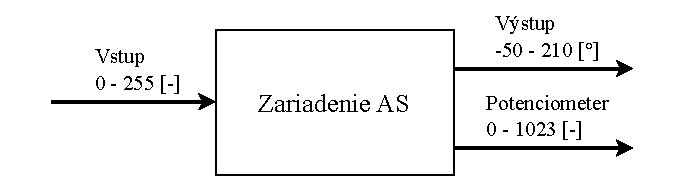
\includegraphics{AS_system.pdf}
        }

        \figcaption{
            Signály systému AS.
        }
        \label{LMOT_sch1}
    }%vbox

\end{center}


\begin{center}

    \vbox{%


        \makebox[\textwidth][c]{%
            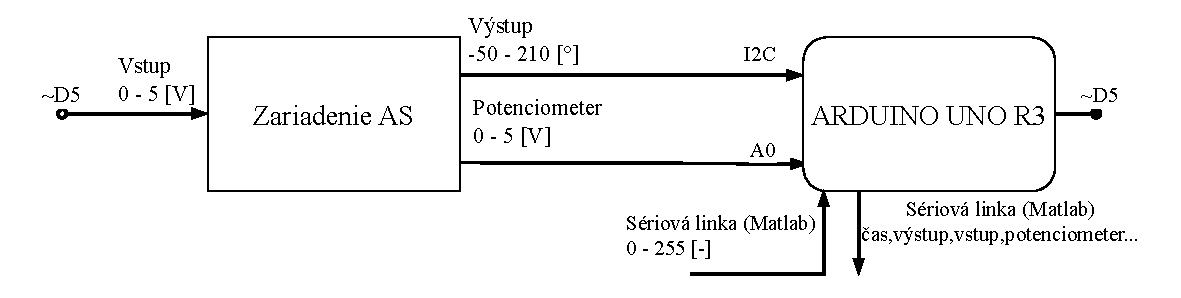
\includegraphics{AS_system_pinout.pdf}
        }

        \figcaption{
            Schéma pripojenia laboratórneho zariadenia AS ku GPIO pinom Arduino UNO R$3$.
        }
        \label{AS_sch2}
    }%vbox

\end{center}

Na obr. \ref{AS_sch2} môžeme vidieť, že A$0$ je analógový vstup potenciometra, $\sim$D$5$ je fyzický výstup akčného zásahu na logickej úrovni vo forme \emph{PWM} (\href{https://docs.arduino.cc/learn/microcontrollers/analog-output/}{Pulse-Width Modulation}), I$2$C slúži na odčítanie uhlovej polohy ramena.



\section{Fotografie}

Zoznam fotografií:

\begin{itemize}
    \item Obr. \ref{IMG_6874_toPDF}: Celkový pohľad na laboratórne zariadenie LMOT.
    \item Obr. \ref{IMG_6922_toPDF}: Motor a tachodynamo.
    \item Obr. \ref{IMG_6941_toPDF}: Elektronické obvody zariadenia.
    \item Obr. \ref{IMG_6931_toPDF}: Predný panel so svorkami a potenciometrom.
\end{itemize}





\noindent
\vbox{%

    \makebox[\textwidth][c]{%
        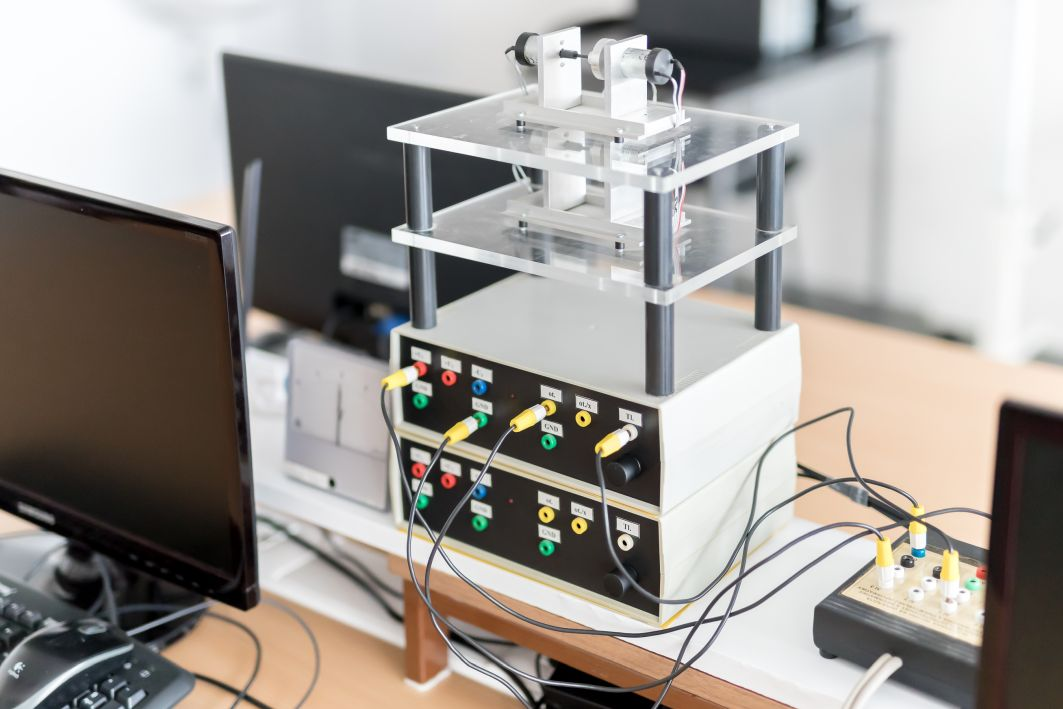
\includegraphics{IMG_6874_toPDF.jpg}
    }

    \figcaption{
        Celkový pohľad na laboratórne zariadenie LMOT.
    }

    \vspace{12pt}

    \label{IMG_6874_toPDF}
}%vbox



\noindent
\vbox{%

    \makebox[\textwidth][c]{%
        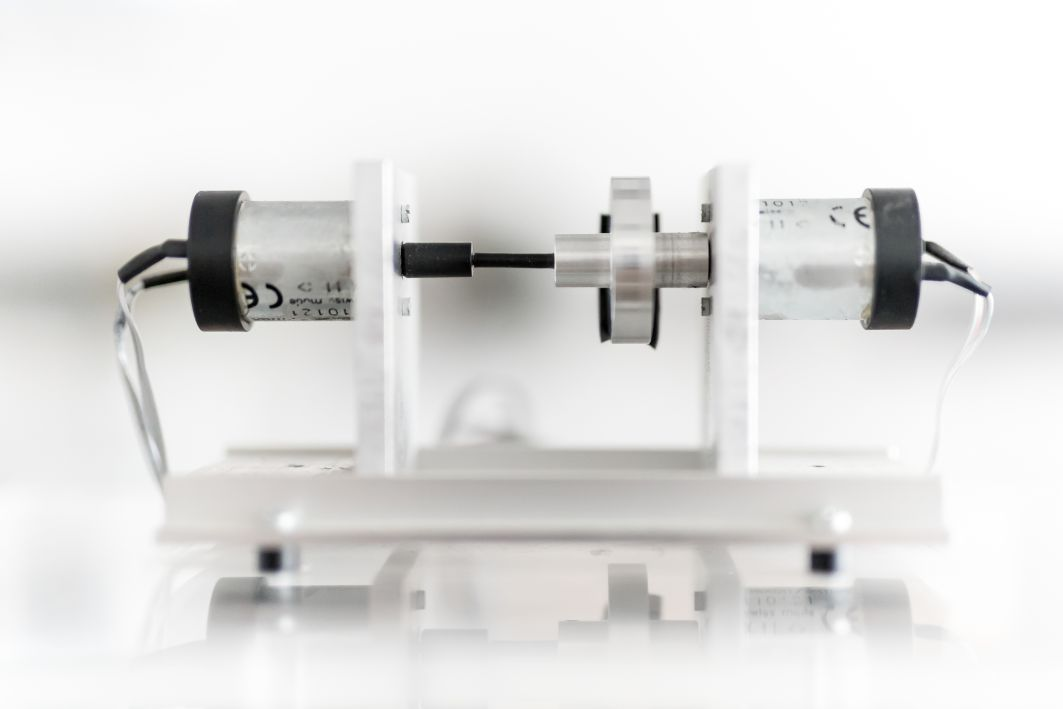
\includegraphics{IMG_6922_toPDF.jpg}
    }

    \figcaption{
        Motor a tachodynamo.
    }

    \vspace{12pt}

    \label{IMG_6922_toPDF}
}%vbox




\noindent
\vbox{%

    \makebox[\textwidth][c]{%
        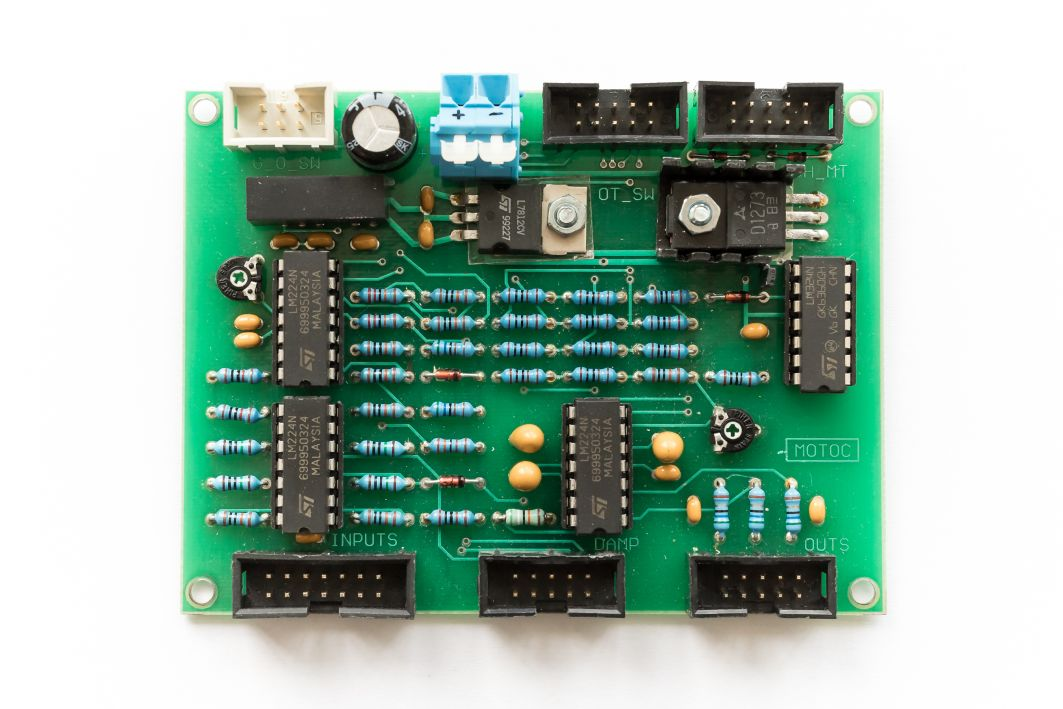
\includegraphics{IMG_6941_toPDF.jpg}
    }

    \figcaption{
        Elektronické obvody zariadenia.
    }

    \vspace{12pt}

    \label{IMG_6941_toPDF}
}%vbox




\noindent
\vbox{%

    \makebox[\textwidth][c]{%
        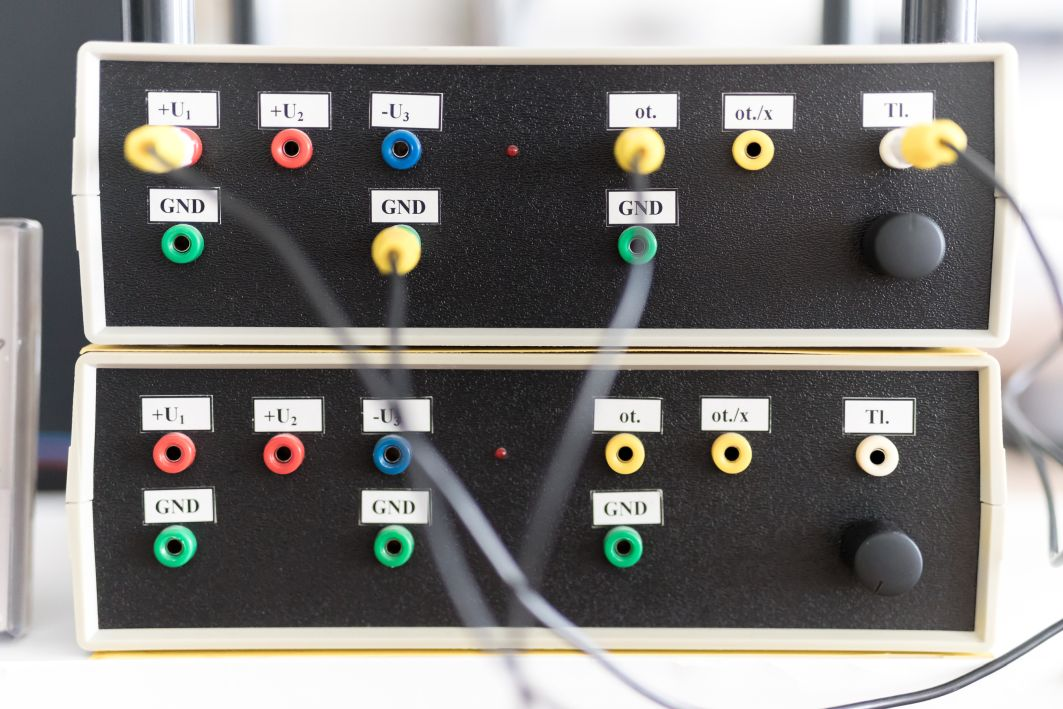
\includegraphics{IMG_6931_toPDF.jpg}
    }

    \figcaption{
        Predný panel so svorkami a potenciometrom.
    }

    \vspace{12pt}

    \label{IMG_6931_toPDF}
}%vbox

























































% -----------------------------------------------------------------------------

\end{document}

% -----------------------------------------------------------------------------